\chapter{Решење проблема применом алгоритма моделовања тема }

Проналажење правог одговора на постављено питање може бити изузетно сложен проблем чак и за човека. Оно што је суштински важно за препознавање ваљаног одговора је разумевање \textbf{суштине} односно смисла питања. За разлику од машина, човек на основу знања, уме да наслути тај смисао а самим тим и да препозна адекватан одговор. Међутим, уколико би се пред човека ставило питање из области о којој он нема никаквог знања ( не разуме значење речи) или је на језику који не разуме, врло је вероватно да би препознавање правог одговора било јако непоуздано. 
Са друге стране, немогуће је не запитати се шта заправо представља прави одговор на постављено питање. Данас је можда лакше него икада поставити питање и у кратком времену добити велики број одговора од различитих корисника. Учесници конверзације не морају нужно бити стручњаци из области које се тиче питања. Исто тако, велики број одговора, иако су наизглед адекватни, наилазе на осуду стручне популације. Дакле, потребно је извесно време, у коме долазо до комуникације међу различитим корисницима ( давање оцена се може сматрати комуникацијим) да би се \textbf{закључило} шта је прави одговор. 
Сајтови који су служили као извор података су управо описаног карактера. Дакле, одговори на поствањено питање се оцењују од стране заинтересованих корисника и након неког времена са великом прецизношћу се може рећи који је адекватан одговор на постављено питање. Према томе, подаци који су овде разматрани јако су зависно од :

\begin{itemize}
\item атрактивности теме којом се баве - што је тема популарнија то ће већи број корисника бити укључен у давање и оцењивање одговора. Самим тим, може се сматрати да атрактивније теме имају поузданије одговоре
\item природе питања - на нека питања се може одговорити врло кратко - (на пример где се ПМФ налази у Крагујевцу ) док друга питања захтевају опширне одговоре (нпр. детаљан опис историје Крагујевца или препричано књижевно дело)
\end{itemize}

У правом одговору не морају нужно да се нађу речи из питања. Исто тако, не мора постојати законитост између дужине питања и одговора. Према томе, не постоји \textbf{алгоритам} којим се може закључити који је адекватан одговор а да се при томе не укљичи додатно експертско знање. 

Основна идеја овог рада је испитивање да ли се и у којој мери вештачно знање које се добија применом алгоритма моделовања тема може употребити за селектовање правог одговора без убацивања додатног експертског знања.


\section{Опис решења}

Идеја решења је изградња \textbf{модела тема} над свим одговорима чиме би се добио истрениран модел који поседује знање о том скупу докумената. Под знањем се подразумева расподела тема над документима као и расподела речи унутар тема. Основна предпоставка је да се при постављању питања то знање може употребити како би се селектовао тачан одговор. Даље сe претпоставља да су  питање и одговор  највероватније из истих области ( једна или више ) односно да говоре о истим темама. Овде је важно напоменути да теримн \textbf{област} или \textbf{тема} више није упоредив са човековим схватањем тема или области. Обзорим да је број тема који се у истраживању користио јако велики - од 100 до 2000 - и да тема није ништа друго до скуп речи као и да у систем није укључено никакво додатно експретско знање, ово напомена је сасвим очигледна.

Селектовање правог одговора вршено је мерењем \textbf{сличности} између постављеног питања и свих одговора. Онај одговор који је \textbf{најсличнији} постављеном питању, одабира се као тачан одговор на постављено питање. Обзиром да је познато који одговор припада ком питању, рад програма је једноставно проверити и измерити.

За мерење сличности питања и одговора коришћено је неколико метода које се разликују  по прецизности, брзини рада и меморијским захтевима. 


Идејни ток решења може се представити  дијаграмом као на слици 5.1:

\begin{figure}[H]
    \centering
   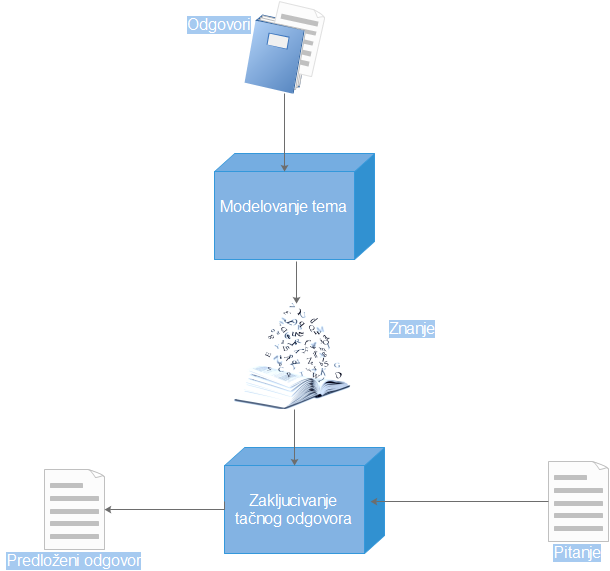
\includegraphics[scale=0.9]{./Slike/slika37.png} 
	\caption{Ток решења}
	\label{fig:slika1}
\end{figure}


\section{Мерење сличности}

Мерење сличности је од суштинске важности за одабирање одговора на поствањено питање. Она утиче на прецизност решења, брзину извршавања, меморијске захтеве итд. У раду су испитане три мере сличности од којих је мера заснована на вероватноћи дале најбоље резултате.



\subsection{Косинусна сличност}

Један од излаза алгоритама тема је и расподела тема по документима. Такође, за сваки нови документ, могуће је предвидети расподелу по темама. Дакле, пошто се вектор расподела по темама увек може направити, корисно их је искористити као меру сличности два документа.

Вектор расподеле по темама, дужине n, може се замислити  као права у n-димензионаланом простору. Дакле, вектор питања и вектор одговора могу се замислити као две праве у n-димензионаланом. Што су те две праве "`ближе"' једна другој, односно што је угао између њих ближи 0, то су питање и одговор сличнији. 
Пошто се ради о расподелама, максимална вредност коју може да узме нека координата овако дефинисаног вектора је 1, док је минимална вредност 0, што значи да се обе праве налазе у првом квадранту. Дакле, максимални угао који два вектора могу да граде је 90 степени и , у смислу косинуссне мере, означава да су документи потпуно различити.
Близина праве питања и праве одговора означава сличну расподелу по темама. Ако се узме у обзор полазна претпоставка да питање и одговор "`говоре о"' истим темама, постаје јасно због чега се угао између ових правих може узети за меру сличности два документа.

Ради илустрације, следи један прилично упрошћен и нереалан пример. 
Нека је скуп свих могућих речи састављен од три речи : \textit{reč1,reč2,reč3} и нека су дате три реченице састављене од поменутих речи : \textit{rečenica1, rečenica2,rečenica3}. 
Дате реченице могу се графички представити као праве ( Слика 5.2)

\begin{figure}[H]
    \centering
   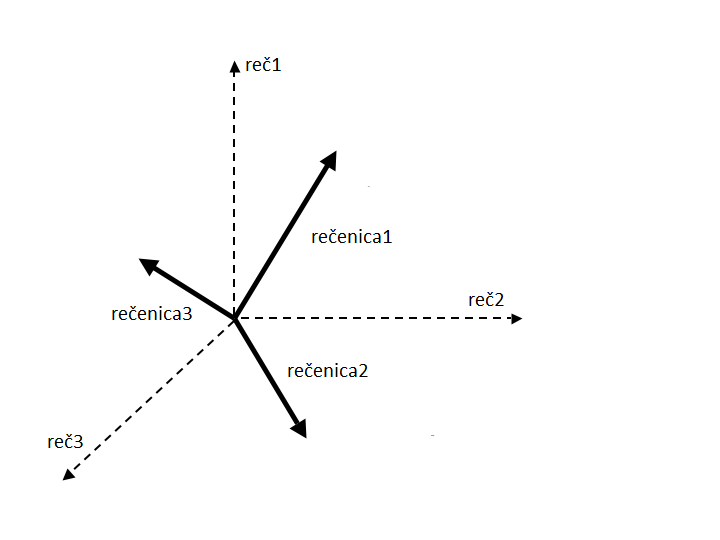
\includegraphics[scale=0.3]{./Slike/kosinusna.png} 
	\caption{Графички приказ косинусне сличности}
	\label{fig:slika1}
\end{figure}

Угао између сваке две праве представља меру сличности реченица.

Уместо мерења угла између два вектора, практичније је мерити косинус тог угла. 
Косинус угла који заклапају два вектора може се одредити следећом формулом :


$$ cos\theta = \frac{\overrightarrow{a}\cdot \overrightarrow{b}}{\Vert\overrightarrow{a}\Vert\overrightarrow{b}\Vert} $$


Претходна формула следи директно из дефиниције \textbf{скаларног произвида} два вектора.



\subsection{Мерење сличности према лексичкој и тематској сличности}

Поред теметске сличности докумената, и лексичка сличност може бити важна. На пример, уколико се у одговору појављују исте речи као и у питању, \textbf{вероватније} је да је тај одговор ближи тачном одговору  него одговор који нема заједничких речи са питањем. Наравно, могу се наћи примери у којима ово не важи. Али, исто тако, могуће је пронаћи примере у којима одговор и питање нису тематски слични - нпр. питање је уско специјализовано док је одговор теметски недефинисан. Према томе, знајући да обе мере сличности не морају увек да гарантују селектовање правог одговора, уз одговорајући ризик, може се испитати утицај комбинације ове две мере на одабир  одговора. 

Поставља се питање на који начин измерити лексичку сличност два документа тј. питања и одговора. Једно од решења би било једноставно бројање истих речи. Међутим, како је циљ испитати утицај \textbf{комбинације} лексичке и теметске сличности, ово решење се не може прихватити као добро. Разлог томе је што је лексичка сличност два документа измерена на овај начин \textbf{увек константна} док се теметска сличност докумената разликује зависно од параметара модела. 	

Други начин мерења лексичке сличности докумената може се добити мерењем лесичке сличности \textbf{тема}.
Пошто се тема математички представља као функција расподеле над скупом свих речи, то сигурно за сваку реч из документа постоје вероватноће са којима свака тема садржи дату реч. Према томе, за сваки документ је могуће саставити $K$ вектора, где је $K$ укупан број тема, при чему $i$-ти вектор садржи вероватниће припадања речи документа  $i$-тој теми. \footnote{Ово се може гарантовати за сваку реч из одговора обзиром да је над скупом свих одговра изграђен модел. Међутим, може се догодити да се у питању појави реч која не постоји у корпусу модела. Вероватноће те речи у свим темама је тада 0} Формалније $i$-ти вектор се може записати као :

\begin{equation}
p_q^{(i)} = p(w_q \mid i,\phi^{(i)})
\end{equation}

при чему је скуп речи документа дат са  $w_q = (w_1,w_2,..,,w_{|q|})$ док је $\phi^{(i)}$ расподела речи унутар  $i$-те теме. 
Дакле, вектор $p_q^{(i)}$ се формира тако што се за сваку реч из документа пронађе вероватноћа припадања те речи  $i$-тој теми тј. важи да је 
$p_q^{(i)} = (\phi_{w_1}^{(i)},\phi_{w_2}^{(i)} ... ,\phi_{w_|q|}^{(i)})$

Нека је одабрана тема  $i$. Да би се измерила лексичка сличност питања и одговора унутар ове теме, потребно је формирати описане векторе за оба документа. Димензије ова два вектора треба да буду исте и једнаке укупном броју различитих речи у корпусу. При томе, вероватноће оних речи из корпуса које не припадају документу ће у  векторима бити постављене на нулу.  Исто тако, треба водити рачуна да редослед навођења речи ( тј. њихових вероватноћа) у оба вектора буде исти. То значи да ако је нпр. вероватноћа речи \textit{математика} у првом вектору наведена на 3. позицији, тада се на 3. позицији у другом вектору налази такође вероватноћа за реч \textit{математика}. 

Сличност ова два вектора може да се мери на више начина. У раду је коришћена косинусна мера сличности док је у раду \cite{tm2} коришћена Јенсен-Шенонова сличност.

Дакле, лексичка сличност два документа у $i$-тој теми може се представити као :

$$
W(p_{pitanje}^{(i)},p_{odgovor}^{(i)}) = kosinusna_slicnost(p_{pitanje}^{(i)},p_{odgovor}^{(i)})
$$

Укупна лексичка сличност питања и одговора се може дефинисати као :

$$
slicnost_1(pitanje,odgovor) = \frac{1}{K}\sum_{k=1}^K W(p_{pitanje}^{(k)},p_{odgovor}^{(k)})
$$


На овај начин је измерена лексичка мера сличности између питања и одговора. Даље, потребно је дефинисати тематску сличност питања и одговора. Она се дефинише као косинусна сличност расподеле тема унутар питања и одговора ( већ опшисана косинусна мера сличности). Дакле:

$$
slicnost_2(pitanje,odgovor) =kosinusnaSlicnost(\theta_pitanje,\theta_odgovor))
$$

Коначно, сличност питања и одговора се дефинише као :

$$
slicnost(pitanje,odgovor) = slicnost_1(pitanje,odgovor)*slicnost_2(pitanje,odgovor)
$$

Ова мера је у пракси показала јако добре резулате. Међутим, битан недостатак јој је јако велика сложеност. Најпре, за свако питање и за сваки одговор потребно је проћи кроз све теме. Ово је већ сложеност $O(n^3)$ која је неприхватиљива у оваквој врсти проблема. Поред временске сложености, и просторна сложеност овог решења није мала. Наиме, за сваку тему мора се чувати (или стално изводити) расподела по свим речима. Величина корпуса може бити јако велика, па је ове структуре готово немогуће чувати у меморији. 
Због велике сложености, ова мера није испитана детаљно као косинусна мера, па су резултати добијени овом мером прилично непоуздани и оквиирни. 
Она није погодна за решавање оваквих типова проблема где величина уланог скупа може достићи и 20 000 докумената. Међутим, при мањем броју докумената, њена просторна и временска сложеност може да се компензује прецизношћу која се њоме добија. Подробнија испитивања ове мере нису рађена у  раду а више о једној варијанти ове мере може се наћи у \cite{tm2}.

\subsection{Мерење сличности према предвиђеној вероватноћи}

Главни резулатати алгоритма моделовања тема су две расподеле - расподела речи по темама и расподела тема по документима. Ове две расподеле могу да се употребе како би се одредила сличност два документа.

Нека је дат документ $D$ и нека су познате $\theta_D$ -расподела тема унутар тог документа и $\phi$- расподеле речи унутатар свих тема. Тада се вероватноћа припадања неке речи $w$ документу $D$ може изразити као :

\begin{equation}
P_{lda}(w \mid D) = \sum_{z=1}^{K} P(w \mid z)P(z \mid \theta_D) 
\end{equation}


при чему : \\

$ P(w \mid z)$ означава вероватноћу речи $w$ унутар теме $z$. Обзиром да речи са различитим вероватноћама припадају различитим темама и да је хиперпараметар Дирихлеове расподеле за расподелу речи над темама $\beta$, ова вероватноћа се изражава као условна, под условом $z$ и $\beta$. Хиперпараметар $\beta$ се подразумева, обзиром на начин како је модел направљен, тако да се и при писању може изоставити.\\
$P(z \mid \theta_D)$- означава вероватноћу са којом се тема $z$ јавља у документу $D$. Из сличних разлога као и код претходног чиниоца, ова вероватноћа се изражава као условна под условом $\theta_D$ и $\alpha$,  стим што се $\alpha$ подразумева па се и не пише.

Дакле, формулом (5.2) може се прерачунати колико је вероватно да реч $w$ припада документу $D$. Ово се још може посматрати и као вероватноћа да је реч $w$ генерисана документом $D$.

Имајући ово у виду, може се сада дефинисати и вероватноћа да скуп речи припада документу  $D$, и то као :

\begin{equation}
P_{lda}(Q \mid D) = \prod_{w \in Q} p_{lda}(w \mid D) 
\end{equation}

Претходна једнакост уставри дефинише вероватноћу да је скуп реч генирасан документом $D$. Узимајући специјално да је тај скуп речи питање које се поставља систему, једнакост се може протумачити и као вероватноћа генерисања поставњеног питања из датог одговора. \textbf{Вероватноћу генерисање} треба схватити као могућност извлачења речи питања из одговора.  Што је ова вероватноћа већа, већа је и могућност да питање и одговор говоре о истим стварима те да посматрани одговор може бити тражени одговор на постављено питање.

Вероватноћа припадања речи $w$ неком     документу $D$ се, поред формуле (5.2) може посматрати и из угла класичне вероватноће. Дакле, веровтаноћа да ће се реч $w$ наћи у      документу $D$ једнака је укупном броју појављивања речи $w$ у том документу подељено са укупним бројем речи документа, односно :

\begin{equation}
P(w \mid D) = \frac{f_{w,D}}{|D|}
\end{equation}

где је $f_{w,D}$ број појављивања речи у документи док је $|D|$ укупан број речи у документу.

Обзиром да реч $w$ може бити било која реч, није нужно да она припада документу $D$. Дакле, може да се деси да ова вероватноћа буде 0. Имајући у виду формулу (5.3), овако нешто је апсолутно неприхватљиво, поготово код дужих питања. На пример, уколико постоји само једна реч која се налази у питању а не налази у одговору, док се осталих  ,рецимо, 100 поклапају, то би резултовало вероватноћом  0 за генерисање питања из текста одговора. Овако нешто, наравно, не може да буде тачно.
Овај проблем може се решити увеђењем \textbf{псеудо појављивања}. 
Псеудо појављивања представљају број појављивања који се узима као подразумевани уколико се реч питања не налази у тексту одговора. На овај начин свакој речи питања ће се доделити нека вероватноћа, која није 0, али је ипак довољно мала да ће велико непоклапање речи између два документа одразити на резултат. Псеудо појављивања могу се увести на више начина. У конкретном раду, формула (5.4) замењена је са формулом (5.5).

\begin{equation}
P(w \mid D) = \frac{f_{w,D} + \mu\frac{c_{w_i}}{|C|}}{|D|+\mu}
\end{equation}

где је\\
$\mu$ параметар који се експериментално одређује и представља псеудо појављивање\\
$C$ је ознака укупног корпуса речи добијеног из свох одговора
\\
$c_{w_i}$ - појављивање речи у корпусу.

Ни овакво решење није без мане. Наиме, и даље може да се деси да вероватноћа (5.3) буде једнака 0. То је случај када се у тексту питања појављује реч која није нашла \textbf{ни у једном} од одговора. Међутим, овакви случајеви су ретки, поготово код већих скупова улазнох података. Међутим, ако се то и деси, таквој речи, уместо вероватноће рачунете на било који од описаних начина, се додељује вредност хиперпараметра $\beta$. Ова вредност узета је зато што се у алгоритму моделовања тема, управо она додељује свим речима у оквиру свих тема у нултој итерацији. Та вредност сигурно није нула, али је довољно мала како би утицала на резултат.

Једнакостима (5.5) и (5.2) дефинисане су вероватноће припадања неке речи одређеном документу али са различитим физичким смислом. Једнакост (5.2) дефинише тематску сличност док једнакост (5.5) дефинише лексичку сличност. Међутим, ове две сличности не морају увек да буду подједнако важне, иако су обе значајне. Због тога би требало да постоји могућност контролисања удела са којим ове две сличности улазе у крајњу процену сличности. У конкретном раду, овај проблем решен је додвањем додатног параметра $\lambda$. Што је његова вредност већа, то је лексичка сличност докумената важнија и обрнуто.

Помениуте вероватноће могу се уклопити тако да заједно граде меру сличности. У конкретном раду, вероватноћа генерисања речи из текста дата је са:

\begin{equation}
P(w \mid D)  = \lambda(\frac{f_{w,D} + \mu\frac{c_{w_i}}{|C|}}{|D|+\mu}) + (1-\lambda)(\sum_{z=1}^{K} P(w \mid z)P(z \mid \theta_D))
\end{equation}

Мера укупне сличности два документа дата се и даље рачуна преко (5.3).
За вредности парамтера $\lambda$ и $\mu$  могу се узети било које вредности, уз ограничење $\lambda \leq 1$. За потребе рада, експериментално су одређене врености $\mu = 200$ и $\lambda = 0.2$.
